\documentclass[12pt, twoside]{article}
\usepackage[letterpaper, margin=1in, headsep=0.5in]{geometry}
\usepackage[english]{babel}
\usepackage[utf8]{inputenc}
\usepackage{amsmath}
\usepackage{amsfonts}
\usepackage{amssymb}
\usepackage{tikz}

\usepackage{pgfplots}
\pgfplotsset{width=9cm,compat=1.9}

\usepackage{venndiagram}

\usepackage{graphicx}
\usepackage{enumitem}
\usepackage{multicol}

\usepackage{fancyhdr}
\pagestyle{fancy}
\fancyhf{}
\renewcommand{\headrulewidth}{0pt} % disable the underline of the header

\fancyhead[LE]{\thepage}
\fancyhead[RO]{\thepage \\ Name: \hspace{4cm} \,\\}
\fancyhead[LO]{BECA / Dr. Huson / IB Mathematics\\* Unit 5: Polynomial functions\\* February 2020}

\begin{document}
    \subsubsection*{5.8 Homework: Graphing and interpreting quadratic functions}

For each function, first factor it (always show this step), then state the roots using the form, ``$x=3,4$'' (or whatever the values are).
\begin{enumerate}

\begin{multicols}{2}
    \item   $f(x)=x^2+7x+12$ \vspace{6cm}
    \item   $f(x)=x^2+13x+12$ \vspace{6cm}
    \item   $f(x)=x^2-4x-12$ \vspace{6cm}
    \item   $f(x)=2x^2-10x-12$ \vspace{6cm}
    \item   $f(x)=-3x^2+6x-3$ \vspace{6cm}
    \item   $f(x)=\frac{1}{2}x^2+2x+2$ \vspace{6cm}
\end{multicols}

\newpage
\subsubsection*{Completing the square}

Rewrite the function in vertex form, $f(x)=(x-h)^2+k$. Include the step showing the $(-\frac{b}{2a})^2$ term.
    \begin{multicols}{2}
    \item   $f(x)=x^2-6x+11$
    \item   $f(x)=x^2+8x+9$
    \end{multicols} \vspace{6cm}

Expand the function from vertex form to standard form, $ax^2+bx+c \text{ where } a, b, c \;  \epsilon \; \mathbb{R}$. Then factor the result and state the roots. Sketch the function, labeling the intercepts with values and the vertex as an ordered pair.
\item   $f(x)=(x-2)^2-9$
  \begin{flushright}
  \begin{tikzpicture}[scale=0.35]%[scale=0.635]
    \draw [thick, ->] (-10.2,0) -- (10.4,0) node [below right] {$x$};
    \draw [thick, ->] (0,-10.2)--(0,10.4) node [left] {$y$};
  \end{tikzpicture}
  \end{flushright}

\newpage
\subsubsection*{Graphing quadratics}
\item Graph the function $f(x)=-x^2-4x+5$. You may use a graphing calculator rather than factoring the function and completing the square.\\*[0.25cm]
Label the scales with at least a few values. Mark the vertex as an ordered pair and label each intercept with its value.

\begin{center}
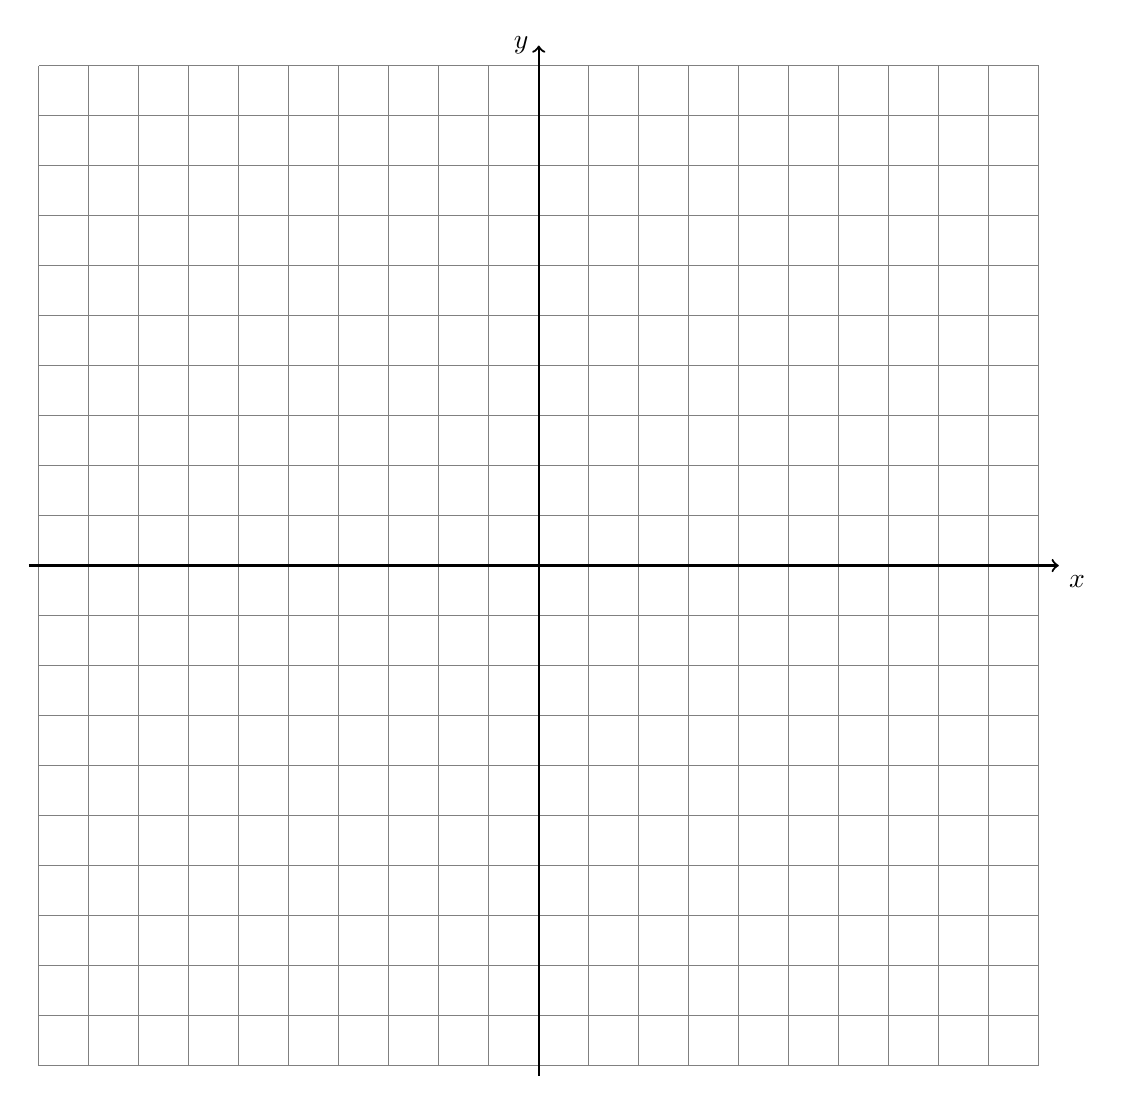
\begin{tikzpicture}[scale=0.635]
  \draw [help lines] (-10,-10) grid (10,10);
  \draw [thick, ->] (-10.2,0) -- (10.4,0) node [below right] {$x$};
  \draw [thick, ->] (0,-10.2)--(0,10.4) node [left] {$y$};
\end{tikzpicture}
\end{center}

\newpage
\subsubsection*{Model situations with quadratic functions}

Use a graphing calculator to view the graph and a table of values for the following function:
\[h(x)=-\frac{1}{225}x^2+\frac{2}{3}x\]
where $h(x)$ represents the height of an object and $x$ it's horizontal position.\\*[5pt]
Make a table of values to the left of the graph, below. Include key values. Graph the function over domain where $h(x) \geq 0$. Use a horizontal scale of 1 square equals 10 units and vertical scale of 1 square equals 2.5 units. Label the intercepts and vertex.\\*[1cm]

\begin{flushright}

\begin{tikzpicture}
  \draw [help lines] (0,0) grid (10,10);
  \draw [thick, <->] (0,10.2) node [left] {$y$}
       -- (0,0) -- (10.2,0) node [below right] {$x$};
\end{tikzpicture}
\end{flushright}
           
\end{enumerate}
\end{document}